\documentclass[journal]{IEEEtran}

\usepackage{amsmath,amssymb}
\usepackage{graphicx}
\usepackage{booktabs}
\usepackage{array}
\usepackage{cite}
\usepackage{url}
\usepackage{balance}

\graphicspath{{figures/}}
\newcommand{\model}{Student A02}

\title{Design and Analysis of Lightweight Diffusion Models for Efficient Image Inpainting}

\author{\IEEEauthorblockN{Md Minhajul Islam, Kazi Tazrian Mon, and Nur Ibne Kawsar Zitu}
\IEEEauthorblockA{Department of Electrical and Computer Engineering\\
North South University, Dhaka, Bangladesh}}

\begin{document}
\maketitle

\begin{abstract}
The advantages of diffusion models in image inpainting tasks are evident; however, their computation costs are often high for real-time applications. This paper introduces a latent diffusion framework for efficient image inpainting, where we aim to achieve satisfactory reconstruction quality with a significant decrease in computational burden. Starting from a baseline diffusion model, we experimentally explore ways of simplifying its architecture through depth reduction, channel dimensionality reduction, and simplified conditioning. Using these experiments, we propose a lightweight latent-space U-Net model named Student A02 and train it using a teacher-student knowledge distillation approach under a frozen Stable Diffusion 2 U-Net teacher. We conduct experiments on the CelebA dataset, measuring our model with FID, PSNR, SSIM, and LPIPS scores on masked regions. Our Student A02 model yields an FID of 46.95, PSNR of 21.22 dB, SSIM of 0.871, and LPIPS of 0.088 using only 6.7 million parameters and taking around 0.63 seconds per image for inference. In contrast, Stable Diffusion 2 uses approximately 1.29 billion parameters and requires around 5--14 seconds per image depending on evaluation settings. Therefore, our proposed model is about 190 times lighter and 10--20 times faster than Stable Diffusion 2 while maintaining acceptable reconstruction quality.
\end{abstract}

\begin{IEEEkeywords}
diffusion models, image inpainting, latent diffusion, teacher-student knowledge distillation, Stable Diffusion 2
\end{IEEEkeywords}

\section{Introduction}
\subsection{Background and Motivation}
Image inpainting refers to a computer vision task associated with generating missing and distorted areas of an image to produce a seamless output with high visual fidelity. This approach can find numerous applications in image restoration, content removal, content creation, and other domains. However, existing approaches, based on traditional methods like diffusion-based partial differential equation solutions and patches, generally fail to maintain consistency at a global semantic level.

The recent progress in deep learning allowed developing various models based on neural networks to perform image inpainting. In particular, models based on generative approaches have achieved remarkable results recently. One of the most powerful techniques is the approach based on diffusion processes which enables modeling of a data distribution through progressive denoising. Stable diffusion models have proved superior results compared to GANs, among others, with higher stability and visual realism.

On the other hand, diffusion-based models suffer from significant practical issues, the most notable of which includes high computation cost due to high complexity, large size, and the need for multiple sampling steps required to generate the final output. State-of-the-art diffusion models for image inpainting involve billions of parameters and take multiple seconds per input image during inference. Hence, these models cannot be used for real-time tasks, as well as deployment in limited-resource environments like mobile devices.

Several attempts to mitigate these issues were proposed recently. In particular, various methods include architectural simplifications, latent space modeling, and sampling optimization. However, while the improvements in computational efficiency have been demonstrated, there is still considerable room for improvement in balancing between the efficiency and image quality produced.

Inspired by this gap, this project will design and experiment with new lightweight diffusion models to reduce computational costs without substantial loss in visual quality of generated images. Using various architectural modifications and distillation-based training, it will attempt to achieve better balance in efficiency and quality of inpainted images.

\subsection{Purpose and Goal}
First and foremost, the key objective of this research is related to the creation, analysis, and implementation of a lightweight model for inpainting images based on the Stable Diffusion framework, which would be able to combine the minimal amount of computations with sufficient quality of reconstruction. Although the performance of current algorithms for image inpainting based on the Stable Diffusion model is quite high, those solutions are still associated with the relatively large volume of the model and need a considerable time for carrying out the inference procedure. For that reason, the proposed project offered developing a small-size latent diffusion model.

As for the steps required for accomplishing this objective, several experiments were carried out. At first, the initial model of diffusion and its operation principles were thoroughly examined and investigated. Furthermore, various approaches to modifying the architecture of the initial Stable Diffusion model were explored including changing its depth, number of channels, and types of conditioning.

Once all the necessary experiments were carried out, the main emphasis was made on the development of small-size latent diffusion model named Student A02 model. The key idea behind this model was the use of a relatively simple architecture of U-Net operating within the latent space. Moreover, it was decided to utilize the approach of distillation where the teacher would be Stable Diffusion 2 model.

Based on the obtained results, there are several main conclusions that can be made:
\begin{itemize}
  \item Creation of a small-size latent diffusion model for image inpainting
  \item Carrying out experiments aimed at studying the impact of model simplification on its performance
  \item Development of distillation model intended to enhance performance
  \item Using multiple criteria such as FID, PSNR, SSIM, LPIPS for evaluating model performance
  \item Creation of visualization tool comparing small-size model to large one
\end{itemize}
Thus, one could say that the key feature of the novelty of the project is associated with the fact that the application of proper distillation technique and architecture is vital for improving the efficiency of lightweight models.

\section{Research Literature Review}
One major advancement in the area of image inpainting has been made possible by diffusion-based generative models, which show impressive results when generating semantically consistent and visually realistic reconstructions. Unfortunately, in spite of all the strengths these techniques demonstrate, they bring along considerable computational problems making their real-world application impractical. Analysis of the recent research shows that there is an obvious trade-off between the quality of image inpainting and computational costs.

Lugmayr et al. propose RePaint, a training-free approach to diffusive inpainting, which enhances the original reverse diffusion process with several rounds of injection of pixel-wise information according to a resampling schedule \cite{lugmayr2022repaint}. The method allows for achieving generalization across any type of mask distribution, but its efficiency decreases drastically as it requires hundreds of diffusion steps to be performed. In experiments on datasets such as CelebA-HQ and ImageNet, RePaint manages to reach excellent visual quality with an LPIPS score reaching as low as 0.028 for narrow masks. However, due to its poor efficiency, this method fails to be suitable for use in real time.

In an attempt to solve this issue, Corneanu et al. propose a technique called LatentPaint, based on diffusive inpainting implemented in the latent space \cite{corneanu2024latentpaint}. By using the simple and efficient propagation mechanism, LatentPaint reduces considerably the computational effort needed for inpainting. In particular, its performance in terms of visual quality can be assessed via the FID score equal to 7.06 achieved for CelebA-HQ. Yet, LatentPaint does not solve the problem of high computational costs as it uses multi-step diffusion sampling and therefore needs multiple denoising operations.

An attempt to find ways to optimize efficiency is made by Zhang et al., who apply the skip-step DDIM sampling and coarse-to-fine denoising scheme in the context of diffusive image inpainting \cite{zhang2024minutes}. In this way, inference time is considerably shortened as the image is generated at low resolution and then refined in later steps. As a result, the performance of the proposed algorithm can be estimated in terms of SSIM reaching as high as 0.918 and competitive FID values. However, the architecture of this model adds to its sampling complexity, besides it is only applicable in GPU environments.

On the contrary, MI-GAN is a more lightweight GAN-based inpainting model suggested by Sargsyan et al., with depthwise separable convolutions and knowledge distillation \cite{sargsyan2023migan}. This allows for reducing the number of parameters to 5.95 million with an FID value of about 11.83. However, due to the limitations of the GAN framework, GAN-based models are less stable and diverse compared to diffusion models in terms of their reconstruction capacity.

Likewise, Zhao et al. suggested MobileDiffusion, which attempts to make diffusion models run effectively on mobile platforms by using step reduction and simple architectural design \cite{zhao2024instant}. According to their experiments, this model can enable diffusion models to have almost real-time performance, with the minimum inference latency of 238 milliseconds. Yet, while MobileDiffusion performs quite well in generating images from texts, there is no comprehensive experimental assessment with regard to image inpainting task in terms of PSNR and SSIM.

Apart from architectural designs, other approaches focused on optimization techniques to reduce the computation costs of diffusion models. For example, Buzovkin et al. attempted to develop a lightweight decoder for latent diffusion models, suggesting that substituting the vanilla VAE decoder with some alternative design will decrease the decoding time without changing the diffusion process \cite{buzovkin2025decoder}. Even though this method provides improvements in decoding process, it does not solve the problem with the costliness of the denoising backbone or the entire sampling process.

According to a survey made by Chen et al., current diffusion models are able to generate high-quality images thanks to sophisticated architecture designs and multilevel optimization training \cite{chen2024survey}. Nevertheless, these improvements tend to increase the computational requirements of these models, which makes them impractical. Moreover, according to an empirical study conducted by Wang et al., advanced diffusion models such as DesignDiffusion produce highly realistic generated images \cite{wang2025designdiffusion}.

In general, there are multiple issues that could be pinpointed from the current state of affairs. First of all, diffusion-based approaches to image inpainting strongly depend on multi-stage sampling, which inevitably leads to significant inference time delays. Secondly, most of the state-of-the-art models require high-power computation, which makes them unsuitable for edge computing and other limited-resources platforms. While some approaches are trying to tackle this problem via reduced sampling time or simplified network structure, they tend to add up to complexity themselves. Finally, GAN-based lightweight approaches offer faster inference and parameter usage but still cannot cope with stability, diversity, and realism of reconstruction provided by their diffusion counterparts. There is also an evident lack of unified approach that efficiently implements latent space usage and distillation from teacher to student networks in current research.

This way, there is an obvious research gap in terms of lightweight yet efficient diffusion-based image inpainting model, which would not sacrifice inference time and architecture complexity for satisfactory reconstruction quality. This research is driven by such a problem statement and aims at architectural simplification along with distillation from teacher to student model.

\section{Methodology}
\subsection{System Design}
The architecture proposed in this paper is based on a lightweight Latent Diffusion Model for Image Inpainting by adopting model optimization approaches such as teacher-student distillation techniques. The design is intended to greatly decrease computation cost but still preserve reasonable reconstruction performance. Specifically, the entire process can be divided into three phases: preprocessing and latent encoding, diffusion-based training with teacher guidance, and inference through reverse diffusion followed by decoding.

\begin{figure*}[t]
  \centering
  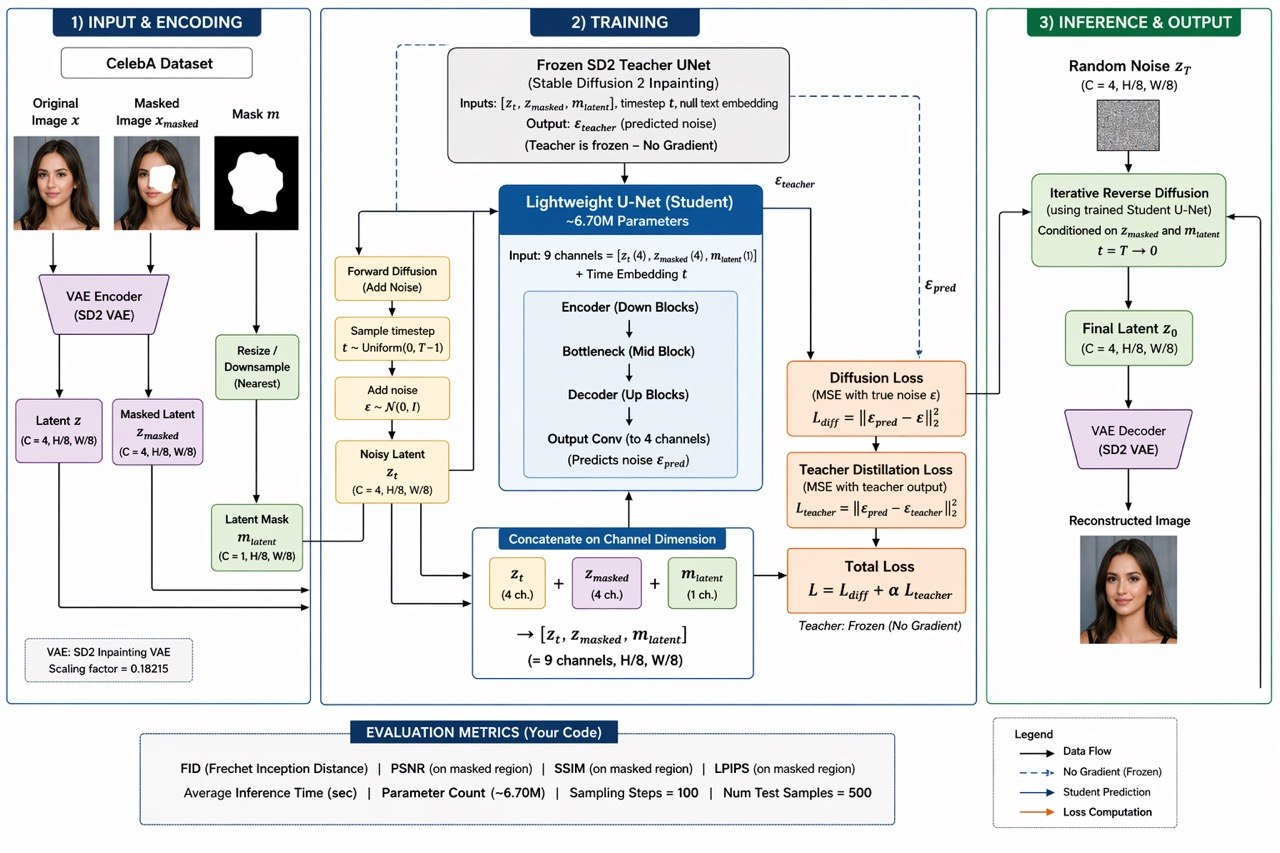
\includegraphics[width=0.96\textwidth]{student_a02_architecture.jpeg}
  \caption{Proposed lightweight latent diffusion inpainting architecture for Student A02.}
  \label{fig:architecture}
\end{figure*}

\subsubsection{Input Preparation and Mask Conditioning}
Our system takes an RGB image as input:
\begin{equation}
x \in \mathbb{R}^{3\times H\times W}.
\end{equation}
where H and W represent the height and width of the image. A corresponding binary mask is also used:
\begin{equation}
m \in \{0,1\}^{1\times H\times W}.
\end{equation}
In this mask, $m=1$ represents the region to be inpainted or removed, while $m=0$ represents the region that should be preserved. The masked image is generated by removing the masked region from the original image:
\begin{equation}
x_{masked}=x\odot(1-m),
\end{equation}
where $\odot$ denotes element-wise multiplication.

\subsubsection{Latent Space Encoding}
To improve computational efficiency, the system operates in latent space instead of directly processing the image in pixel space. A pretrained Variational Autoencoder (VAE) from Stable Diffusion 2 is used to encode both the original image and the masked image into compressed latent representations:
\begin{align}
z &= 0.18215\times VAE_{encoder}(x),\\
z_{masked} &= 0.18215\times VAE_{encoder}(x_{masked}).
\end{align}
For an input image resolution of $256\times256$, the encoded latent representation becomes:
\begin{equation}
z\in\mathbb{R}^{4\times32\times32}.
\end{equation}
This means the spatial resolution is reduced by a factor of 8, which significantly lowers the computational cost. The binary mask is also resized to match the latent resolution:
\begin{equation}
m_{latent}=Resize(m).
\end{equation}
Nearest-neighbor interpolation is used during resizing so that the mask remains binary and does not introduce unwanted intermediate values.

\subsubsection{Conditioned Model Input}
The conditioned input to the student model is formed by concatenating three latent-space components along the channel dimension: the noisy latent $z_t$, the masked-image latent $z_{masked}$ and the resized latent mask $m_{latent}$. Since $z_t$ contains 4 channels, $z_{masked}$ contains 4 channels, and $m_{latent}$ contains 1 channel. Thus, the conditioned input becomes:
\begin{align}
u_t &= Concat(z_t,z_{masked},m_{latent}),\\
u_t &\in \mathbb{R}^{9\times32\times32}.
\end{align}
This 9-channel conditioning allows the model to identify the corrupted region while also using the surrounding visible context for accurate reconstruction.

\subsubsection{Forward Diffusion Process}
During training, the forward diffusion process is applied to the latent representation to gradually corrupt it with Gaussian noise. A timestep is first sampled uniformly as:
\begin{equation}
t\sim Uniform(0,T-1).
\end{equation}
Noise is then added to the latent representation according to the diffusion schedule:
\begin{equation}
z_t=\sqrt{\bar{\alpha}_t}\,z+\sqrt{1-\bar{\alpha}_t}\,\epsilon.
\end{equation}
Where, $\epsilon\sim\mathcal{N}(0,I)$ represents Gaussian noise, and $\bar{\alpha}_t$ is the cumulative noise schedule at timestep $t$. In this work, the total number of timesteps is set to $T=1000$ timesteps. This process progressively transforms the clean latent representation into a noisy version. As a result, the model learns to reverse this corruption process by predicting and removing the added noise, which is essential for reconstructing the original image during inference.

\subsubsection{Lightweight Student Model Architecture}
The backbone of our architecture is a lightweight U-Net based denoising network called Student A02. This network is created to be less computationally intensive yet still retain its necessary encoder-decoder architecture needed for the diffusion-based reconstruction process. It comprises an initial convolution layer, which takes in the 9-channel input, two down sampling layers, a bottleneck layer with residual processing, two up sampling layers, and a convolution layer to output 4 channels of noise.

Noise prediction for the student model can be expressed as:
\begin{equation}
\epsilon_{pred}=f_{\theta}(u_t,t),
\end{equation}
where $u_t$ is the conditioned input and $t$ is the timestep embedding. The final Student A02 model contains approximately 6.7 million parameters, making it significantly smaller than the full Stable Diffusion 2 pipeline.

\subsubsection{Teacher-Student Distillation Framework}
The Stable Diffusion 2 U-Net, which has been trained before, is utilized as the teacher model and stays unchanged in training. Thus, the teacher serves as the guide while not increasing inference cost. The noise is predicted by the teacher as:
\begin{equation}
\epsilon_{teacher}=\mathbf{f}_{SD2}(\mathbf{u}_t,t).
\end{equation}
Training of the student is done through a combination of both diffusion loss and teacher distillation loss. Diffusion loss acts on the student by ensuring that the predictions for the added noise in the forward diffusion process are correct, while teacher loss ensures that the student follows the strong teacher model:
\begin{align}
L_{diff}&=\lVert\epsilon_{pred}-\epsilon\rVert_2^2,\\
L_{teacher}&=\lVert\epsilon_{pred}-\epsilon_{teacher}\rVert_2^2,\\
L_{total}&=L_{diff}+\alpha L_{teacher}.
\end{align}
Where $\alpha=0.1$. This balanced loss allows the model to learn both the true noise distribution and the structural guidance from the teacher model.

\subsubsection{Reverse Diffusion and Image Reconstruction}
During inference, the model starts from random latent noise sample:
\begin{equation}
z_T\sim Normal(0,I).
\end{equation}
The Student A02 model thus denoises the latent representation using the reverse diffusion technique as follows:
\begin{equation}
z_T\rightarrow z_{T-1}\rightarrow\cdots\rightarrow z_0.
\end{equation}
As opposed to the training phase, no teacher network such as Stable Diffusion 2 participates in the inference phase. The lightweight Student A02 model suffices for the task, which reduces computational cost and enables faster image generation. Once the reverse diffusion process is over, the final latent vector output $z_0$ is converted to an image through the Stable Diffusion 2 VAE decoder:
\begin{equation}
\hat{x}=VAE_{dec}\left(\frac{z_0}{0.18215}\right).
\end{equation}
The output of this process will be the final reconstructed image, with the masked area replaced by generated data that fits within the visible portion of the image.

\subsubsection{System Characteristics}
The efficiency of the proposed method is achieved through latent-space processing, lightweight model design, mask-conditioned input, and teacher-student distillation. First, latent-space processing reduces the spatial resolution by 8$\times$, making the method more efficient than direct pixel-space processing because it requires less computation. Second, the U-Net network in the Student A02 model contains only 6.7 million parameters, compared to approximately 1.29 billion parameters in Stable Diffusion 2.

The smaller parameter size helps improve inference speed and makes the model more suitable for low-resource environments. Moreover, mask conditioning helps the model distinguish between regions that require reconstruction and regions that should remain unchanged. Finally, teacher-student distillation allows the student model to learn structural guidance from the pretrained Stable Diffusion 2 teacher while keeping the teacher frozen during training and removing it completely during inference. Thus, the proposed method achieves a reasonable balance between model size, inference speed, and image reconstruction capability.

\subsection{Dataset, Tools, and Implementation}
As for the data set that was used in this research, it consisted of pictures of aligned faces that compose the famous CelebA data set. This type of images was chosen considering the popularity of face inpainting tasks, as well as the necessity to perform them with high consistency. Finally, for the Student A02 experiment, the CelebA dataset was scaled to $256\times256$ images. The size of its subsets was 3000 training samples, 500 validation examples, and 500 for testing. In order to make sure that a fair comparison between Student A02 and the baseline teacher is performed, the dataset had been used for both.

In order to make sure that realistic conditions for the image inpainting task are created, various types of masks have been considered, such as rectangular, brush-style irregular, center, and blob. This variety is important since the image inpainting process is quite close to a reality, where masks have a tendency to take on any form and appear in accordance with any pattern. In order to adapt these masks to the latent space, all of them are converted to a binary format and scaled to the latent resolution of a diffusion model.

Student A02 is a light U-Net denoising diffusion network working in the latent space. Instead of being fed with $256\times256$ pixels images, this model receives their representation in the latent space of Stable Diffusion 2 VAE. Therefore, images become smaller in their spatial resolution, while computing power required for training and inference is reduced. Student A02 takes nine channels for input (noisy latent, masked-image latent, and mask itself), whereas four channels constitute its outputs (noise vector). Overall model size is about 6.7 million parameters. Stable Diffusion 2 Inpainting was employed as a teacher model and baseline for comparison in this research. Teacher's model gives the best noise prediction instructions to the distillation model. Teacher's model's weights were not trained and frozen during the training process, which means that only a lightweight student model is updated. Stable Diffusion 2 is comprised of around 1.29 billion model parameters (UNet, VAE, text encoder). Large-scale architecture makes this model effective; however, computational resources consumption is too high. Thus, a lightweight student is needed.

Mostly, PyTorch library was employed to develop custom models, train and validate those with custom loops, and use the GPU. Pretrained components of Stable Diffusion 2 architecture (inpainting, VAE, scheduler) were obtained from HuggingFace diffusers library. Libraries like NumPy, PIL, OpenCV, TorchMetrics, and LPIPS were used for image preprocessing and metrics computation. In the final step, Gradio library enabled developing an application interface where users could choose an image, define a mask region, and compare results between student (A02) and teacher models.

Experiments were conducted on cloud-based GPU-enabled computing platforms like Google Colab Pro and Kaggle. NVIDIA A100 GPU resources were needed for heavy training and testing purposes, while T4 GPUs could be used to run some small-scale experiments and validate findings. GPU environments were chosen due to the necessity of conducting repetitive denoising, performing big tensor manipulations, and storing tensors in the GPU memory.

\begin{table*}[t]
\caption{Software Tools}
\label{tab:tools}
\centering
\footnotesize
\setlength{\tabcolsep}{5pt}
\begin{tabular}{p{0.16\textwidth}p{0.24\textwidth}p{0.17\textwidth}p{0.34\textwidth}}
\toprule
Tool & Functions & Other similar Tools & Why selected this tool \\
\midrule
Stable Diffusion 2 / VAE & Converts images to and from latent space & Autoencoder variants & Enables efficient latent-space diffusion \\
DDPM Scheduler & Noise scheduling and reverse denoising & DDIM, PNDM & Standard diffusion scheduler suitable for training \\
TorchMetrics & FID calculation & CleanFID & CleanFID \\
LPIPS & Perceptual similarity measurement & DISTS & Measures perceptual quality beyond pixel-level metrics \\
PIL / OpenCV & Image resizing, masking, and preprocessing & scikit-image & Efficient image processing support \\
Google Colab Pro \& Kaggle & GPU-based training and evaluation & Local workstation & Provides accessible GPU resources \\
Gradio & Interactive deployment interface & Streamlit, Flask & Simple interface for image upload, mask drawing, and model comparison \\
\bottomrule
\end{tabular}
\end{table*}

\subsection{Training and Inference Pipelines}
For training, the PyTorch environment was chosen, and training involves a sophisticated pipeline for latent diffusion models training via teacher-student distillation. The preprocessing of data consists of resizing of input images to $256\times256$ resolution and normalizing them into range $[-1,1]$. Moreover, a binary mask was also resized and produced for each image.

The training sample contains the original image, image with masked areas filled in with pixels of masked area removed, and a binary mask itself. These images were transformed into latent representation using the pretrained Stable Diffusion 2 VAE encoder. It is necessary to note that latent diffusion models require latent scaling by 0.18215 factor.

At every training step, a value for timestep was sampled from 1000-steps schedule. After that, the latent was corrupted with Gaussian noise to produce noisy latent. The next step consists of constructing model input, which consists of concatenating noisy latent, masked latent, and binary mask. They are all concatenated to form a 9-channel input tensor for student model A02.

Then, the result of student model was treated as the predicted noise component. Also, the reference noise component was produced by the pretrained Stable Diffusion 2 UNet model. This teacher model was not involved in training process, however, it is used to calculate teacher distillation loss.

Both diffusion and teacher loss components are used in training process. The first one models a proper noise distribution, while the second one helps transfer the behavior of the teacher to the student model. The loss function contains these two components and is minimized during training by AdamW optimizer with learning rate of $1\mathrm{e}{-4}$.

During the inference process, the Student A02 neural net functions independently without the involvement of the teacher model. The inputs consist of an image and its mask. At first, the preprocessing stage of inputs occurs similarly to that of the training process. Then, a masked image is produced, and both images are fed to the VAE encoder to generate latent representation. Unlike training, inference begins by random sampling of noise in latent space instead of having latent representation as an initial condition.

Then, reverse diffusion occurs iteratively at each time step. Specifically, at each time step, the model generates noise vectors which are then used to diffuse latent representation according to the diffusion schedule. This is repeated until reaching the required number of sampling steps, which usually varies from 50 to 100 based on the desired speed-quality ratio. Finally, the latent representation is decoded using the VAE decoder. Thus, an output image with a completed content in the required area is obtained.

\begin{figure*}[t]
  \centering
  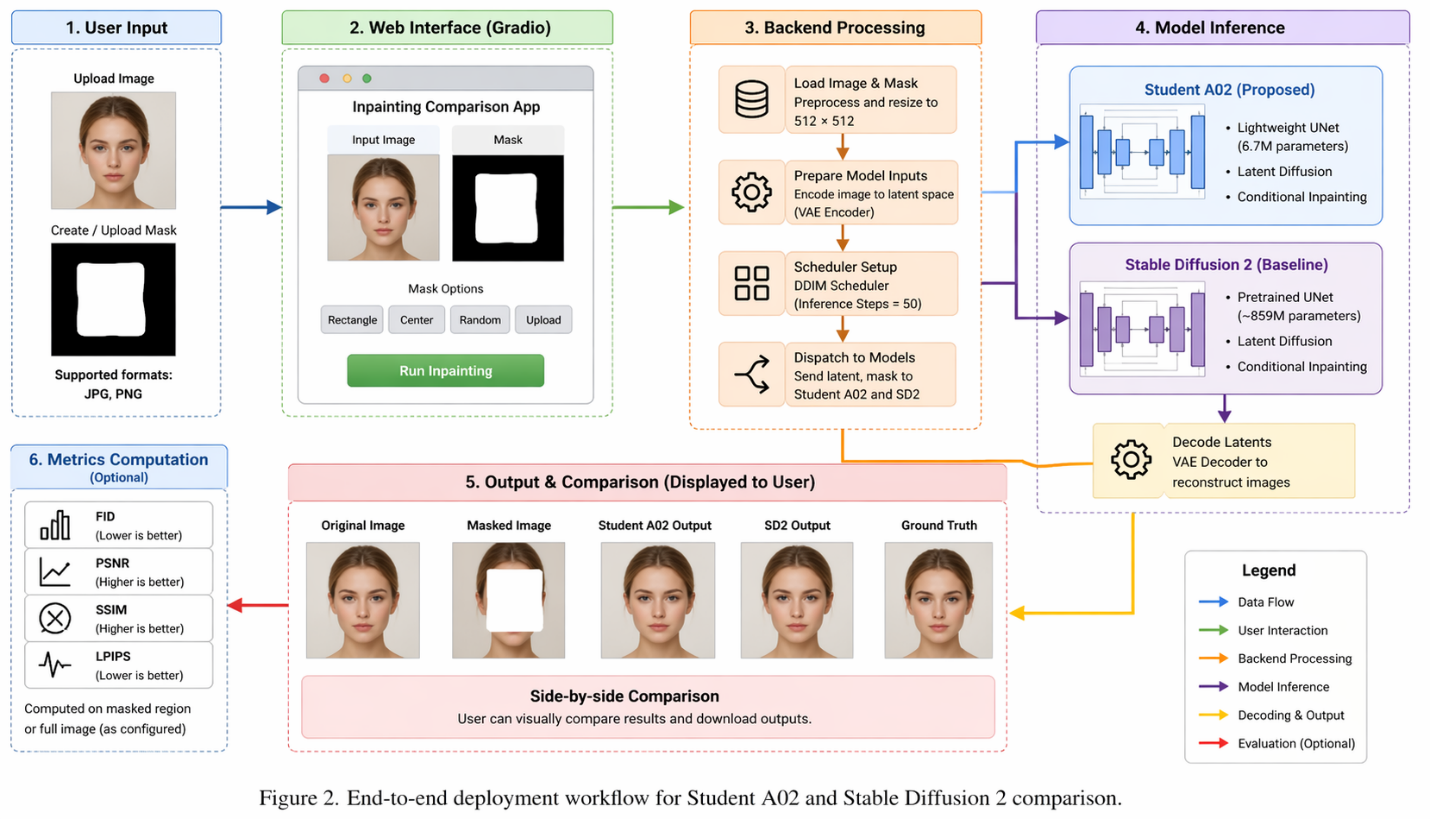
\includegraphics[width=0.92\textwidth]{deployment_workflow.png}
  \caption{End-to-end deployment workflow for Student A02 and Stable Diffusion 2 comparison.}
  \label{fig:deployment}
\end{figure*}

\subsection{Deployment and System Integration}
For the purpose of demonstrating the practical usability of the proposed model, a deployment framework based on Gradio is used. The provided deployment allows users to perform real-time image inpainting through the use of a web-based interactive interface. The main functionality of the application can be listed as follows:
\begin{itemize}
  \item Input image uploading
  \item Drawing/uploading a mask to indicate areas to be filled
  \item Specifying the inference model to use (either Student A02 or Stable Diffusion 2)
  \item Comparison panel for visual results
\end{itemize}
The system utilizes both a lightweight version of the proposed model and a more computationally costly stable diffusion model to provide an opportunity to compare outputs obtained via both models. The concept of the model registry is implemented, allowing switching between models, saving settings, and maintaining benchmark data. Such a solution enables flexibility and ensures that new lightweight models can be easily integrated into the system later.

Also, several utility modules are designed to provide preprocessing, masks processing, and size adjustment of images, as well as a proper visualization of results. A special comparison panel is generated with original image, masked image, student and baseline outputs presented visually.

The entire system thus involves the training process, inference, and deployment all together in one framework. The optimized model checkpoints that have been generated during the training process are used in the inference module. Inference and the deployment system are directly connected to each other, which helps them to operate in real time.

Through such a modular architecture, we get:
\begin{itemize}
  \item The possibility of having the training process independent of optimization
  \item The inference process to continue being efficient
  \item The ability to deploy any model without any hassles
\end{itemize}
It is not only the experimental process that can be conducted through our system but also a complete end-to-end framework as well.

\section{Experiments, Results, and Discussion}
\subsection{Initial Exploration and Ablation Study}
The first part of the project revolved around the evaluation of diffusion models behavior and finding possible areas for improvement. The DDPM algorithm was trained using the CIFAR-10 dataset, and a number of architectural improvements were applied in an ablation study. This included reducing depth, removing attention layers, applying depth wise convolution, and reducing channel width. This part of the research did not aim at obtaining the best results but was targeted at analyzing the effect of different improvements on the efficiency of a particular architecture.

\begin{table}[t]
\caption{CIFAR-10 Ablation Study Results}
\label{tab:ablation}
\centering
\footnotesize
\setlength{\tabcolsep}{3.1pt}
\begin{tabular}{lrrr}
\toprule
Model Variant & Parameters & FID$\downarrow$ & Time$\downarrow$ \\
\midrule
Baseline & 28.89M & 59.76 & 0.0126 \\
Depth Reduced & 20.56M & 59.85 & 0.0104 \\
No Attention & 27.05M & 60.11 & 0.0102 \\
Depth wise Conv & 11.67M & 64.54 & 0.0125 \\
Width Half & 7.49M & 65.74 & 0.0083 \\
Best Combined & 2.29M & 87.07 & 0.0070 \\
\bottomrule
\end{tabular}
\end{table}

As seen from the analysis, such adjustments as a reduction of depth significantly reduce the number of parameters without changing the FID score substantially. However, radical compression methods applied to the model result in a decrease in accuracy. This experiment shows that one significant aspect is that efficiency can be improved at minimal quality loss.

\subsection{Training Stability and Structured Evaluation}
After identifying potential improvements in architecture, the next stage involved testing the stability and sustainability of the performance of the model. The models were trained for long periods of time to verify whether depth-reduced models can maintain their performance during extensive training periods.

\begin{table}[t]
\caption{Baseline vs Depth-Reduced Comparison}
\label{tab:stability}
\centering
\footnotesize
\setlength{\tabcolsep}{3pt}
\begin{tabular}{lrrr}
\toprule
Model & Parameters & MACs & FID$\downarrow$ \\
\midrule
Baseline (100 epochs) & 28.87M & 5.107B & 467.91 \\
Depth Reduced (100 epochs) & 20.55M & 5.054B & 474.45 \\
\bottomrule
\end{tabular}
\end{table}

Training for both models was found to be stable. Though the number of parameters in the depth-reduced network is smaller than that in the baseline network, its performance is similar. This means that depth reduction does not affect the learning capabilities.

During this phase, an improved evaluation mechanism was established. This was through standardized testing that involved a large population and uniform testing conditions as opposed to instant evaluations.

\begin{table}[t]
\caption{Structured Evaluation Results}
\label{tab:structured}
\centering
\footnotesize
\setlength{\tabcolsep}{2.6pt}
\begin{tabular}{lrrrr}
\toprule
Model & Params & MACs & FID$\downarrow$ & Time$\downarrow$ \\
\midrule
Baseline & 28.87M & 5.107B & 60.73 & 0.0128 \\
Depth Reduced & 20.55M & 5.054B & 43.83 & 0.0104 \\
\bottomrule
\end{tabular}
\end{table}

Through the improved evaluation process, it was evident that the depth reduction model significantly performed better than the baseline model in terms of FID as well as efficiency.

\subsection{Transition to Real Inpainting Task}
Once the method was validated on CIFAR-10, the project proceeded to a more practical task of image inpainting, utilizing the CelebA dataset. Variants of the model were created to experiment with lightweight designs for conditional reconstruction under a mask condition.

\begin{table}[t]
\caption{Inpainting Model Comparison}
\label{tab:inpainting}
\centering
\footnotesize
\setlength{\tabcolsep}{2.7pt}
\begin{tabular}{lrrrr}
\toprule
Model & Params & MACs & FID$\downarrow$ & Time$\downarrow$ \\
\midrule
Baseline & 53.99M & 9.856B & 135.47 & 0.2306 \\
Variant A & 5.20M & 1.613B & 103.73 & 0.0871 \\
Variant B & 1.73M & 0.488B & 91.75 & 0.0488 \\
\bottomrule
\end{tabular}
\end{table}

Variant B outperforms other variants in terms of performance with lightweight designs, with a decrease in parameters by more than 96\% and a lower FID score.

\begin{figure*}[t]
\centering
\begin{minipage}{0.485\textwidth}\centering
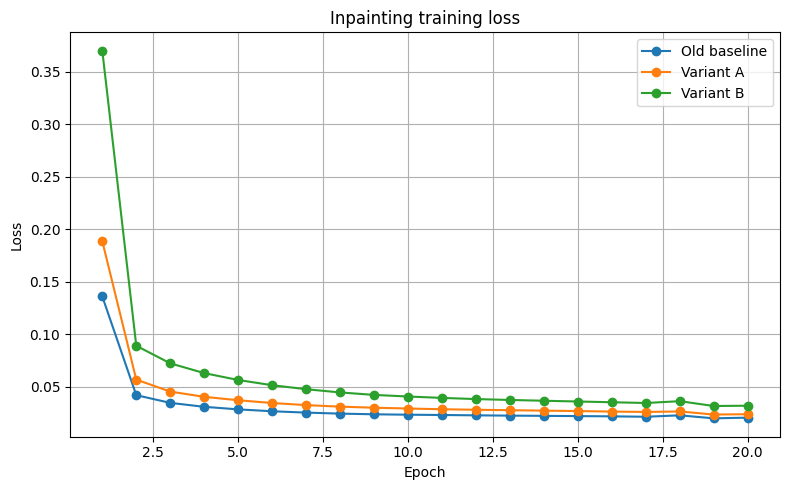
\includegraphics[width=\linewidth]{training_loss.png}
\end{minipage}\hfill
\begin{minipage}{0.485\textwidth}\centering
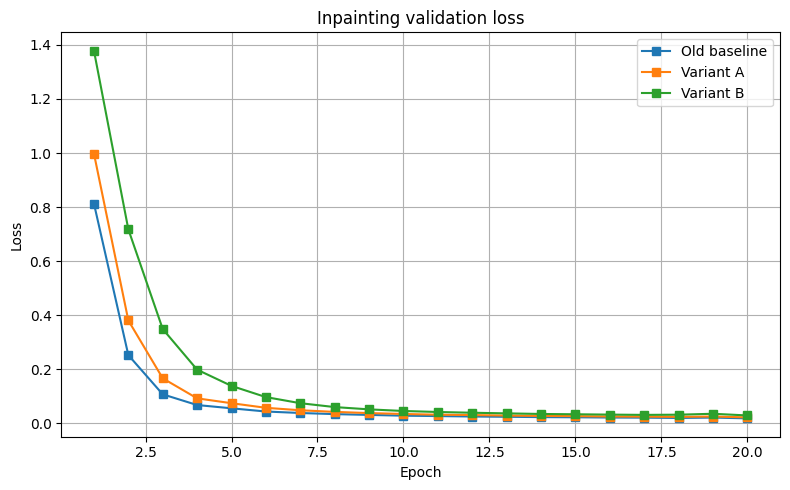
\includegraphics[width=\linewidth]{validation_loss.png}
\end{minipage}
\caption{Training and validation loss curves for CelebA inpainting variants.}
\label{fig:variant-loss}
\end{figure*}

\begin{figure*}[t]
\centering
\begin{minipage}{0.47\textwidth}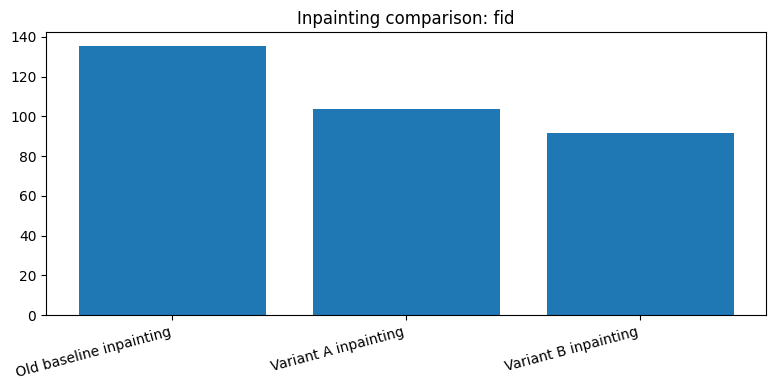
\includegraphics[width=\linewidth]{comparison_fid.png}\end{minipage}\hfill
\begin{minipage}{0.47\textwidth}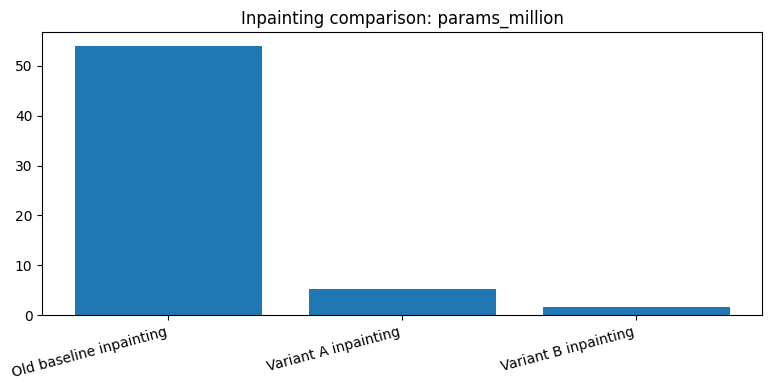
\includegraphics[width=\linewidth]{comparison_params.png}\end{minipage}\\[3pt]
\begin{minipage}{0.47\textwidth}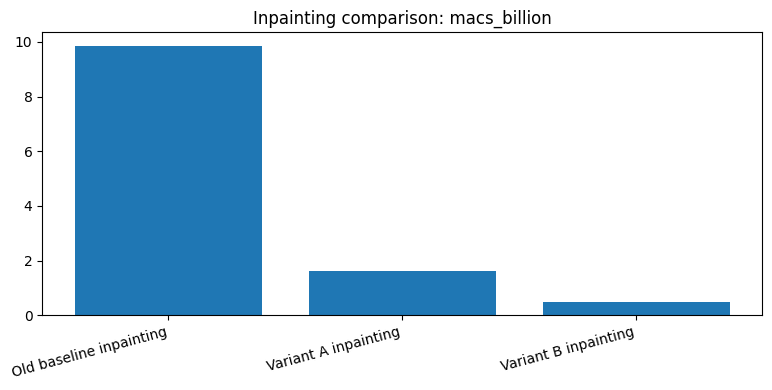
\includegraphics[width=\linewidth]{comparison_macs.png}\end{minipage}\hfill
\begin{minipage}{0.47\textwidth}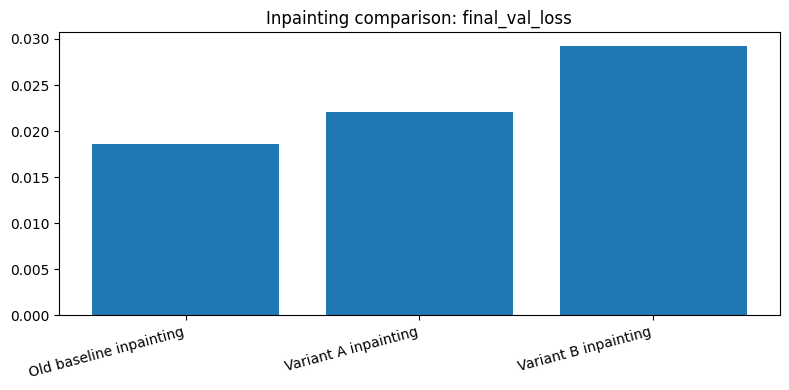
\includegraphics[width=\linewidth]{comparison_validation_loss.png}\end{minipage}
\caption{Performance comparison of baseline, Variant A, and Variant B across FID, parameter count, computational cost (MACs), and validation loss.}
\label{fig:variant-comparison}
\end{figure*}

As seen in Fig.~\ref{fig:variant-comparison}, it can be observed that there is a compromise between the complexity and accuracy of the model. The baseline model achieves the minimum validation loss and has the best reconstruction ability at a much higher computational cost. Meanwhile, Variant A achieves a lower number of parameters and computational costs with comparable performance. Variant B achieves the smallest number of parameters and MACs but suffers from a higher validation loss and poor reconstruction quality.

In the analysis based on the FID score, it can be found that both the variants perform better than the baseline in terms of efficiency but at the expense of perceptual quality. The parameter and MAC analysis proves that the variants significantly reduce the computation cost of the model. Therefore, the above analysis proves that a balance should be maintained between efficiency and reconstruction ability in lightweight diffusion models.

\subsection{Model Training Analysis}
As illustrated by the training curves provided in Fig.~\ref{fig:a02-loss}, the Student A02 model demonstrates a learning performance across 15 epochs. Total loss, diffusion loss, and teacher distillation loss are shown in both training and validation curves. It is noticeable that there is a similarity in the curves in terms of all parameters mentioned, meaning that the learning performance is stable in nature. In addition, there is no large difference between training and validation curves, meaning that there is no problem of overfitting in the proposed approach.

Moreover, there is a clear descending tendency for all mentioned parameters, meaning that there is effective learning happening. Moreover, teacher distillation loss demonstrates stable decreasing, meaning that the learning process from the pretrained Stable Diffusion 2 teacher is effective.

\begin{figure*}[t]
  \centering
  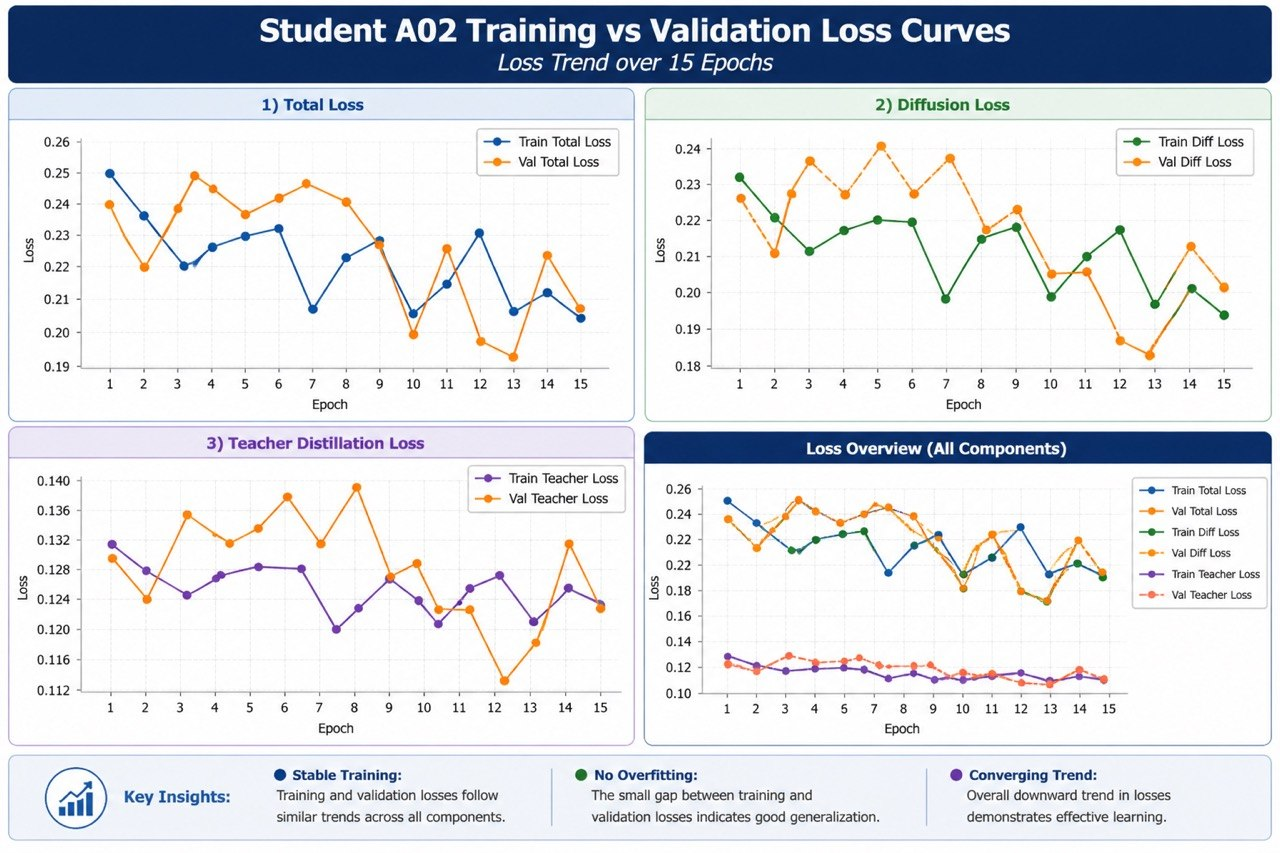
\includegraphics[width=0.92\textwidth]{student_a02_loss_curves.jpeg}
  \caption{Training and validation loss curves of the Student A02 model across different loss components.}
  \label{fig:a02-loss}
\end{figure*}

\subsection{Final Model Development: Student A02}
From all the above discoveries, Student A02 is built using latent diffusion and teacher-student distillation. The model is computationally efficient while maintaining improved reconstruction quality compared to earlier lightweight variants.

\begin{table}[t]
\caption{Student A02 Final Results}
\label{tab:a02-final}
\centering
\footnotesize
\begin{tabular}{lr}
\toprule
Metric & Value \\
\midrule
FID$\downarrow$ & 46.95 \\
PSNR$\uparrow$ & 21.22 \\
SSIM$\uparrow$ & 0.871 \\
LPIPS$\downarrow$ & 0.088 \\
Time$\downarrow$ & 0.637 \\
Parameters & 6.70M \\
\bottomrule
\end{tabular}
\end{table}

The performance of Student A02 shows significant improvement over previously developed lightweight variants. The introduction of teacher-student distillation plays a key role in improving reconstruction quality.

\begin{figure*}[t]
\centering
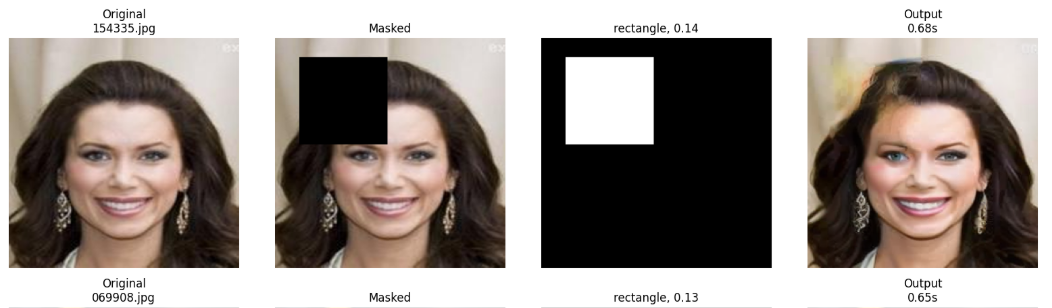
\includegraphics[width=0.82\textwidth]{student_center.png}\\[4pt]
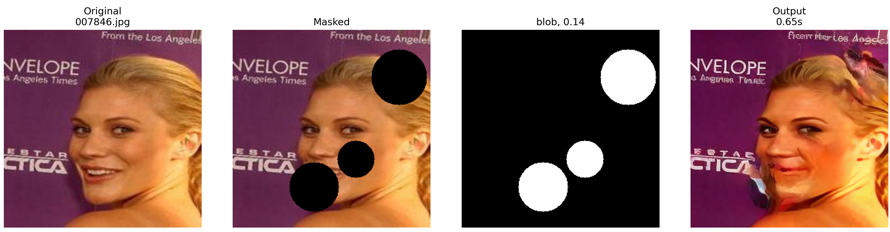
\includegraphics[width=0.82\textwidth]{student_blob.png}\\[4pt]
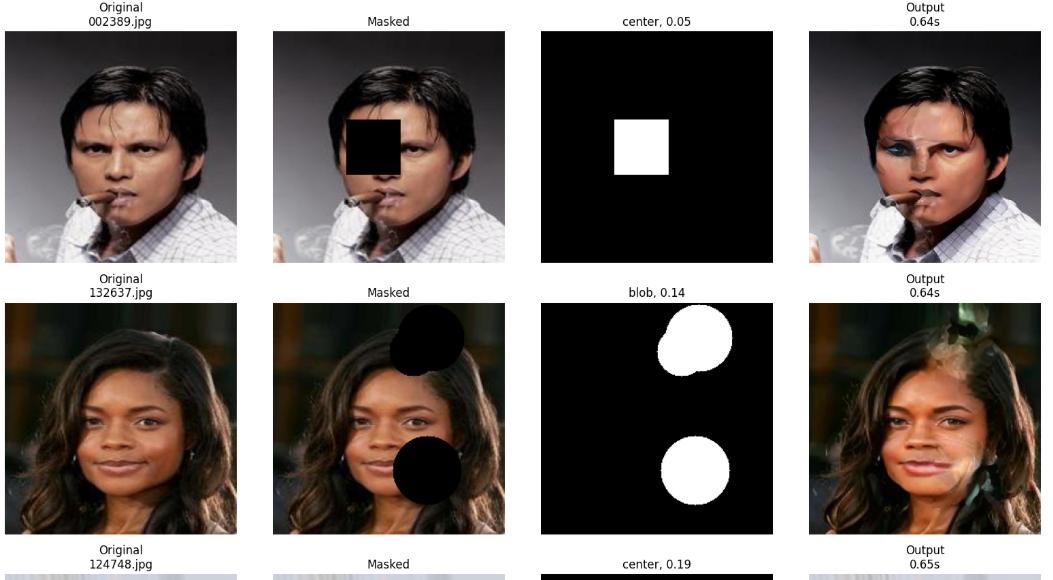
\includegraphics[width=0.82\textwidth]{student_rectangle_blob.png}
\caption{Qualitative comparison showing original images, masked inputs, applied masks, and reconstructed outputs generated by the Student A02 model under different masking strategies (center, blob, and rectangle).}
\label{fig:a02-qualitative}
\end{figure*}

The qualitative results shown in Fig.~\ref{fig:a02-qualitative} indicate the inpainting performance of the Student A02 architecture under different mask designs. The first column is the original image, the second column is the masked image, the third column is the mask itself, and finally, the fourth column is the output of the reconstructed image. It can be observed that the architecture is capable of producing a consistent visual result inside the holes by utilizing the context of the surrounding area. When the masks used are small and regular like the middle or rectangular mask, the generated results produce a coherent image with decent texture consistency. Conversely, when the masks used are irregular, such as the blob mask, there are slight inconsistencies in the texture inside the mask especially when the region is complex like faces.

\subsection{Comparison with Stable Diffusion 2}
\begin{table*}[t]
\caption{Student A02 vs SD2}
\label{tab:sd2}
\centering
\footnotesize
\setlength{\tabcolsep}{7pt}
\begin{tabular}{lrrrrrr}
\toprule
Model & Params & FID$\downarrow$ & PSNR$\uparrow$ & SSIM$\uparrow$ & LPIPS$\downarrow$ & Time$\downarrow$ \\
\midrule
SD2 (512) & 1.29B & 21.97 & 26.85 & 0.94 & 0.04 & 5.79 sec \\
SD2 (256 aligned) & 1.29B & 26.60 & 24.92 & 0.897 & 0.064 & 14.03 sec \\
Student A02 & 6.70M & 46.95 & 21.22 & 0.871 & 0.088 & 0.63 sec \\
\bottomrule
\end{tabular}
\end{table*}

From the results provided in Table~\ref{tab:sd2}, one can see that there is a trade-off between quality and efficiency. The Stable Diffusion 2 model has better quality compared to other models, based on FID, PSNR, SSIM, and LPIPS, due to the size of its architecture and its ability for better text conditioning. Nevertheless, it consumes a lot more computational resources. The suggested Student A02 model, which consists of only 6.7 million parameters, allows for much faster inference with adequate quality.

\begin{figure*}[!t]
\centering
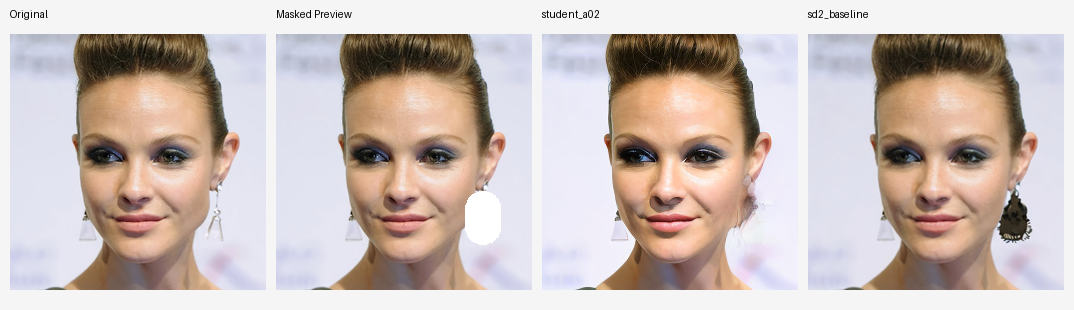
\includegraphics[width=0.68\textwidth]{sd2_compare_01.png}\\[2pt]
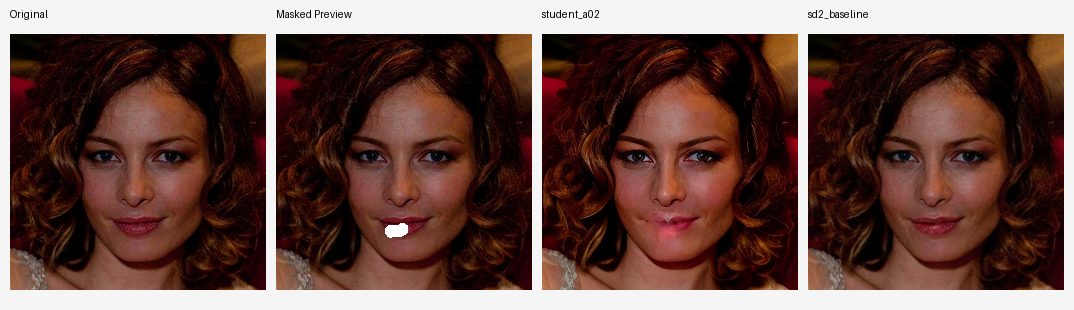
\includegraphics[width=0.68\textwidth]{sd2_compare_02.png}\\[2pt]
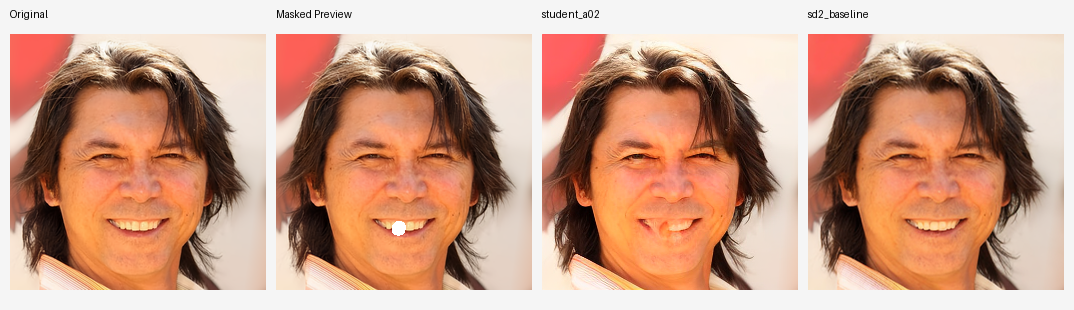
\includegraphics[width=0.68\textwidth]{sd2_compare_03.png}
\caption{Qualitative comparison between Student A02 and Stable Diffusion 2 (SD2) under different masking scenarios, showing original images, masked inputs, and reconstructed outputs (Part 1 of 2).}
\label{fig:sd2-qualitative-a}
\end{figure*}

As illustrated in Figs.~\ref{fig:sd2-qualitative-a} and~\ref{fig:sd2-qualitative-b}, the visual comparison of our proposed Student A02 model against the SD2 baseline demonstrates certain variations between the two architectures. The rows depict the ground truth image, the masked input, as well as the reconstruction outputs from both models. Clearly, SD2 generates relatively sharper and more intricate outputs as a result of having a larger architecture and being conditioned on text input. However, while Student A02 is generating reasonably good reconstructions, it does so at much reduced computational expense compared to SD2. Though some artifacts and texture discrepancies can be seen in certain instances, the structure and identities of the faces are still preserved.

\begin{figure*}[!t]
\centering
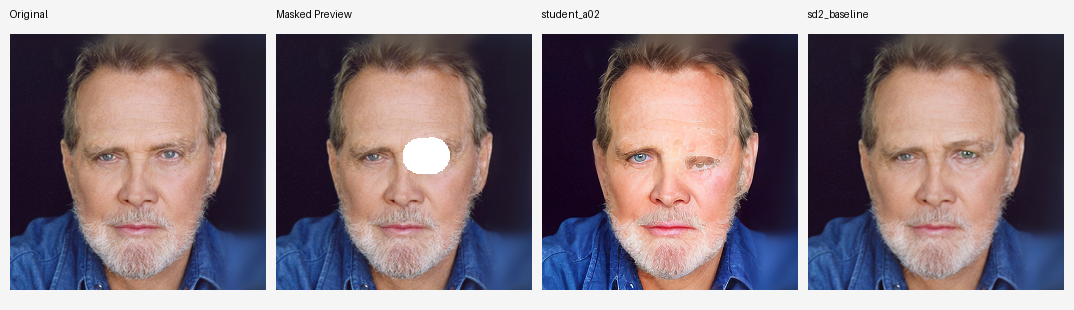
\includegraphics[width=0.68\textwidth]{sd2_compare_04.png}\\[2pt]
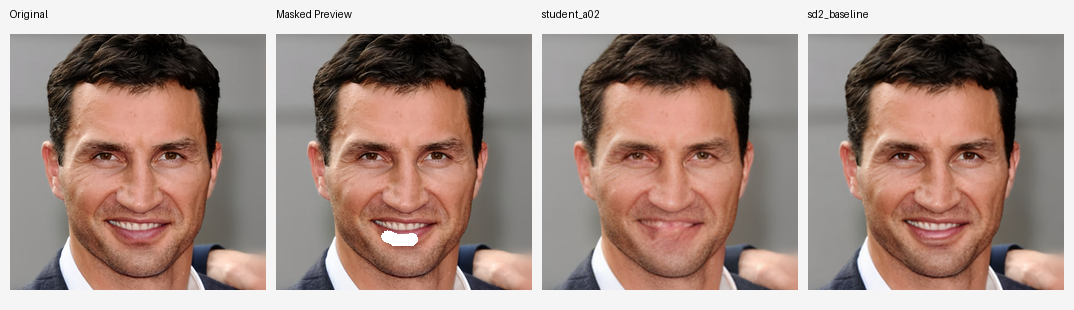
\includegraphics[width=0.68\textwidth]{sd2_compare_05.png}\\[2pt]
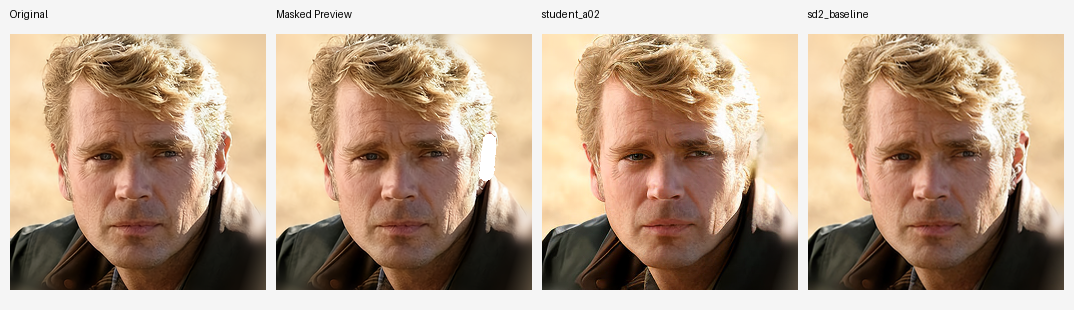
\includegraphics[width=0.68\textwidth]{sd2_compare_06.png}
\caption{Qualitative comparison between Student A02 and Stable Diffusion 2 (SD2) under different masking scenarios, showing original images, masked inputs, and reconstructed outputs (Part 2 of 2).}
\label{fig:sd2-qualitative-b}
\end{figure*}

\subsection{Overall Discussion}
Experimenting results revealed important insights about complexity-efficiency, effectiveness, efficiency, and quality of reconstruction dependencies within diffusion-based image inpainting. The following takeaways were drawn from our research. First of all, according to the results of the ablation study conducted in the first part of the experiment, simplification was shown to lead to lower costs. Among different changes, depth reduction resulted in the most cost-effective way to decrease the number of parameters without deteriorating performance. On the contrary, radical transformations such as compression or channel pruning led to substantial performance drops, indicating redundancy of diffusion models.

In the second part of the experiment, we discovered that carefully designed lightweight models can maintain good performance levels. Experiments conducted in this part demonstrated that there is no contradiction between performance and compactness. Some experiments showed that depth reduction allows reaching better performance than overparameterized models, while others showed similar performance levels in case of proper design.

As far as the third stage is concerned, a critical conclusion regarding the differences between image generation and inpainting tasks was reached. Masked input data and hybrid masking helped to improve inpainting results. Experiments with Variants A and B revealed that lightweight models could generate outstanding results if tailored to solving specific tasks. It turned out that extremely lightweight architectures performed well under certain conditions.

In conclusion, one can see that an increase in model complexity or the introduction of additional losses does not necessarily contribute to better results. In particular, when tuning Students B and C, the use of a perceptual loss and an increase in teacher-loss weight resulted in instability and deterioration of quality. As a result, the simple teacher-student distillation technique applied to Student A02 turned out to be the most reliable and efficient solution.

Thus, as mentioned above, Student A02 is a result of applying this approach to a certain diffusion model. Given all the advantages listed above, Student A02 represents an efficient model with a good performance level. The model works with latent data, uses a compact architecture and employs distillation with a proper loss balance. Even though the student model is not able to surpass a well-tuned, high-capacity teacher, it still performs very well and exceeds other models in terms of efficiency.

Comparing Student A02 with the teacher model, one may notice that the latter consumes more computing power and provides better reconstruction quality while the former works faster and consumes less computing power.

The developed Student A02 model was incorporated in a Gradio deployment framework for visual inference and comparison against Stable Diffusion 2. As demonstrated in Fig.~\ref{fig:deployment} above, the developed framework enables user inputting an image, applying/drawing a mask, and receiving inpainting results from both Student A02 and SD2 models. In turn, the generated outputs are visually presented to the user and can be compared directly.

Thus, this kind of deployment clearly shows that the proposed approach is not confined to offline model performance evaluations. Indeed, since inference in Student A02 model is performed solely using the lightweight network architecture, its outputs are generated faster than those in SD2 model, albeit at a slightly lower reconstruction accuracy level. Consequently, the deployment phase highlights practical applicability of the proposed technique.

\section{Impacts and Resource Considerations}
This section will take a look at the significance of the proposed lightweight diffusion-based image inpainting scheme within the broader context. Various impacts from the social, technological, environmental, and ethical perspectives will be considered. While the primary focus of the research is practical, its outcomes have implications on both practice and future deployment of similar solutions.

\subsection{Societal, Health, Safety, Legal and Cultural Impact}
First, the discussed system offers several significant opportunities and advantages, particularly within the field of digital media, photography, and content creation. In general, the system allows for better editing, manipulation, and reconstruction of visual images and thus provides helpful tools for photographers, graphic designers, and media editors. Moreover, the possibility to edit an image in real-time with the help of a relatively small model increases the number of potential users who have limitations in computing capacities.

Within the health care and research sector, the same approaches of image inpainting can be used for image reconstruction for purposes such as filling gaps in medical images. Although the project deals with faces, the described methodology can also be applied to MRI or CT image reconstruction. However, this application should undergo comprehensive validation to be reliable enough to diagnose.

Concerning safety and ethics, the discussed tool can be used for the purposes of deception or even fraud since inpainting can be used to modify the visual image. Therefore, using the technology requires ethical considerations and possibly the development of ways to detect the manipulation.

From the legal perspective, it is vital to ensure compliance with all applicable legislation when implementing such systems as generative models. Thus, the use of pretrained Stable Diffusion 2 is subject to certain licensing and the application of CelebA dataset according to its conditions.

Finally, from the cultural perspective, the developed system has a tremendous impact on visual content generation and storytelling. With the development of such technologies, new opportunities are created, yet the issues related to authenticity and originality appear.

\subsection{Environmental and Sustainability Impact}
Diffusion models require significant compute capacity, which drives the need to exhaustively train the GPUs and, in consequence, increases the time of execution. This leads to increased electricity consumption and greater environmental costs. Stable Diffusion 2 is one of the most energy-intensive and resource-heavy models.

It is possible to consider the concept of lightweight technology, referring to the development of such model architecture, which would require minimal energy consumption during inference. Student A02 is an example of such model with the number of parameters equal to 6.7 million in contrast to billions in other models. It is worth noting that reduced electricity usage can result from quicker inference as well. Furthermore, lightweight technology can help reduce energy consumption, as it will be possible to train and execute models on cheaper infrastructure. In addition, there will be no necessity to invest in powerful and energy-intensive GPUs anymore.

Nevertheless, it is impossible not to admit that the energy consumption required for training remains considerable, although training is not in the scope of this paper.

\subsection{Resource Optimization}
Another critical aspect of the current research is the importance of resource optimization. To achieve this goal, several measures were implemented:
\begin{itemize}
  \item Datasets were processed using their subsets to train models faster
  \item Saving checkpoints was optimized not to overload storage devices
  \item Processing latent space instead of pixel space decreases computation and memory usage
  \item The final lightweight model reduces the number of parameters significantly, which improves efficiency
\end{itemize}
All of the above allowed performing the research under restricted computational resources while delivering valid results.

\section{Limitations and Future Improvement}
Though we have some limitations in our project still there are still multiple impressive directions to develop and expand further. The important extension would be training DDPM on higher-resolution datasets, which could learn richer semantic features and thus achieve more effective inpainting performance by using CelebA-HQ at resolutions such as $128\times128$ or $256\times256$. Another avenue of extension is in finetuning Stable Diffusion and RePaint; with techniques such as LoRA or Dream Booth-style finetuning on CelebA-HQ masks, the accuracy can be significantly improved while reducing artifacts and thus enhancing the overall quality of generated outputs.

Developing the U-Net architecture also allows for future advancement. Incorporating attention layers or designing the structure of a larger encoder-decoder network would likely provide sharper and more consistent supervised inpainting results. This method would be more developed by integrating modern mask-aware strategies, namely as partial convolutions, PatchMatch, or diffusion assistance, which can solve the limitations and ensure smoother transitions between masked and reconstructed areas.

Since LPIPS is more closely inclined with human perception so we can also implement the evaluation methods by integrating perceptual loss functions such as LPIPS because it would provide a meaningful virtual quality assessment.

\section{Conclusion}
The present project aimed at exploring the feasibility of creating an efficient diffusion-based image inpainting system by performing several ablations, systematic designs, and experiments. It all started from taking a standard DDPM model running on the CIFAR-10 dataset and making several architectural changes, including removing layers, shrinking channels, and disabling attention mechanisms. Consequently, some experiments were performed showing that slight changes lead to considerable reductions in the amount of used parameters while maintaining acceptable quality.

Afterwards, the project moved forward towards structured experimentation with the CelebA dataset. There was a range of lightweight variants created and tested for inpainting. Results showed that it is possible to surpass large baseline architectures through designing small-scale models optimized for inpainting purposes. Particularly, Variant B demonstrated great results by using only 1.73 million parameters while achieving the FID of 91.75.

Then, the idea was taken further by designing the lightweight version based on latent diffusion combined with teacher-student learning framework using Stable Diffusion 2 as the teacher. The resulting Student A02 consists of two elements: latent diffusion algorithm operating in latent space and light U-Net with $\sim$6.7 million parameters.

Finally, the implementation and deployment of an actual image inpainting tool were performed through developing the Gradio application capable of inpainting images and comparing different models used for this purpose. Therefore, it has been shown that a lightweight diffusion-based model for image inpainting can be developed by applying appropriate architectural and learning techniques.

\nocite{biswas2025pixels,buburuzan2025mobi,kim2025rad,yang2023unipaint,wasserman2025paint}
\balance
\bibliographystyle{IEEEtran}
\bibliography{references}

\end{document}
